\documentclass[physics_notes.tex]{subfiles}
\begin{document}
\section{ Aula 03 - 30/03/2023}
\subsection{Motivações}
\begin{itemize}
	\item Resolução de Exercícios.
\end{itemize}
\subsection{Exercício 29 - Tipler}
``Considere a trajetória de dois carros, o Carro A e o Carro B. (a) Existe algum instante para o qual os carros estão lado-a-lado? (b) Eles viajam sempre no mesmo sentido? (c) Eles viajam com a mesma velocidade em algum instante t? (d) Para que t os carros estão mais distantes entre si? (e) Esboce os gráficos de $v\times t$'
\begin{center}
	\begin{tikzpicture}
		\begin{axis}[
				axis lines = left,
				xlabel = \(t\),
				ylabel = {\(x(t)\)},
			]
			\addplot [
				domain=0:10,
				samples=100,
				color=red,
			]
			{7*x/2 + 9/3};
			\addlegendentry{\(\text{Carro B}\)}
			%Here the blue parabola is defined
			\addplot[
				domain=0:10,
				samples=100,
				color=blue,
			]
			{-x^2 + 13*x};
			\addlegendentry{\(\text{Carro A}\)}
			%Here the blue parabola is defined
		\end{axis}
	\end{tikzpicture}
\end{center}
Os carros se encontram lado-a-lado quando os gráficos se cruzam, ou seja, em t = 1s e t = 9s (Tipler mais acurado que meu gráfico.). é notável
quer eles não estão sempre no mesmo sentido, visto que, a partir de 6s, o gráfico do carro B passa a mudar o sentido. Em aproximadamente 5s,
ambos estão com a reta tangente iguais, ou seja, estão com a mesma velocidade, e distância entre eles está maior exatamente no ponto em que as
velocidades estão iguais. Finalmente, seguem os gráficos:
\begin{center}
	\begin{tikzpicture}
		\begin{axis}[
				axis lines = left,
				xlabel = \(t\),
				ylabel = {\(v(t)\)},
			]
			\addplot [
				domain=0:6,
				samples=100,
				color=red,
			]
			{-3*x + 18};
			\addlegendentry{\(\text{Carro A}\)}
			%Here the blue parabola is defined
			\addplot[
				domain=0:6,
				samples=100,
				color=red,
			]
			{5};
			\addlegendentry{\(\text{Carro B}\)}
			%Here the blue parabola is defined
		\end{axis}
	\end{tikzpicture}
\end{center}

\subsection{Exercício 44 - Tipler}
``Um carro viaja em linha reta com $\vec{v} = 80\text{km/h} $ durante $\Delta t_{1}=2.5$h. Depois, $\vec{v_{2}} = 40$km/h, $\Delta t_{2} = 1.5$h. Qual
é o deslocamento total? E qual é a velocidade $\vec{v}$ total?''
\begin{align*}
	 & (a)\quad \Delta x = \Delta x_{1} + \Delta x_{2} = \vec{v_{1}}\Delta t_{1} + \vec{v_{2}}\Delta t_{2}  \Rightarrow \Delta x = 260\text{km.} \\
	 & (b)\quad \vec{v} = \frac{\Delta x}{\Delta t} = \frac{260}{4} = 65\text{km/h}.
\end{align*}

\subsection{Exercício 58 - Tipler}
``Um carro acelera de 48.3km/h para 80.5km/h em 3.70s. Qual a aceleração média?''

Primeiramente, precisamos converter as unidades para medidas iguais. Com isso, note que $\vec{v_1} = 48.3km/h = 13.52m/s, \vec{v_{2}} = 80.5km/h = 22.54m/s$. Assim,
chegamos em
$$
	\vec{a} = \frac{\Delta v}{\Delta t} = \frac{v_{2} - v_{1}}{\Delta t}\approx 2.4\text{m/s}.
$$

\subsection{Exercício 67 - Tipler}
``Um corpo está em uma posição inicial $x_{1}$ com velocidade inicial $\vec{v_{1}}$. Passado um tempo, ele se encontra na posição $x_{2}$ com velocidade $\vec{v_{2}}$. Qual é a aceleração deste corpo?''

Utilizaremos Torricelli. sabemos que
\begin{align*}
	 & (1):\quad x_{1} = 6m, \vec{v_{1}} = 10m/s   \\
	 & (2):\quad x_{2} = 10m, \vec{v_{2}} = 15m/s.
\end{align*}
Deste modo, $v^{2} = v_{0}^{2} + 2a\Delta x \Rightarrow v_{2}^{2} = v_{1}^{2} + 2a(x_{2} - x_{1}) \Rightarrow a \approx 16m/s^{2}$

\subsection{Exercício 72 - Tipler}
``Um parafuso se desprende de um elevador subindo a $v_{0} = 6m/s$. O parafuso atinge o fundo do poço em 3s. (a) Qual era a altura do elevador? (b) Qual é a velocidade do parafuso no chão? Tome g = 9.8 $m/s^{2}$''

Sabemos que $t_{0} = 0s, y(t_{0}) = h, v(t_{0}) = v_{0}.$ Com isso, podemos descrever $y(t) = h + v_{0}t + \frac{1}{2}gt^{2}$. Vamos responder, agora, o item a, isto é, qual é o valor
da altura h? Segue que, em $t=3s, y(t) = 0$. Utilizando a fórmula,
$$
	h = -v_{0}t + \frac{1}{2}gt^{2} = -6 \cdot3 + \frac{1}{2}9.8 \cdot 3^{2} = 26.1m
$$
Com relação ao item (b), vimos que $v(t) = v_{0} + at.$ Deste modo,
$$
	v(3s) = 6 - 9.8 \cdot 3 = -23.4m/s
$$
Indo um pouco além do que foi pedido, analisemos o movimento do parafuso. é possível concluir que o parafuso atingirá a altura
máxima no instante em que $t^{*} = \frac{v_{0}}{g} = 0.6s,$ visto que este momento ocorre quando $v(t) = v_{0} - gt = 0$. Com isso,
conclui-se que a altura máxima é $y(t^{*}) = h + v_{0}t^{*} - \frac{1}{2}gt^{*^{2}} \approx 27.5m.$ No gráfico,
\begin{center}
	\begin{tikzpicture}
		\begin{axis}[
				axis lines = left,
				xlabel = \(t\),
				ylabel = {\(y(t)\)},
			]
			\addplot [
				domain = 0:4,
				color = black,
			]
			{0};
			\addplot [
				domain=0:3,
				samples=100,
				color=red,
			]
			{-9.8*x^2/2 + 6*x + 26.1};
			\addlegendentry{\(y(t)\)}
			%Here the blue parabola is defined
			\addplot[
				domain=0:3,
				samples=100,
				color=blue,
			]
			{27.955};
			\addlegendentry{\(h_{\text{max}} = \frac{dy}{dt} = 0\)}
			%Here the blue parabola is defined
		\end{axis}
	\end{tikzpicture}
\end{center}

\subsection{Exemplo - Aula 06 Vanderlei}
``Suponha que há um trem parado no instante t=0 com aceleração a. Passados 6s, um passageiro chega ao local e observa o trem na posição $x_{trem_{1}}$.
Este passageiro sai correndo com velocidade $v_{0}$ para tentar alcançar o trem. Qual é a velocidade mínima que o passageiro precisa atingir
para alcançá-lo?''

Com relação ao trem, suas condições iniciais são $t_{0} = 0, x_{trem} = 0, v_{trem} = 0,$ tal que $x_{trem}(t) = \frac{1}{2}at^{2}$.
Por outro lado, quanto ao passageiro, quando $t=6s, x_{p} = 0$, de modo que $x_{p}(t) = x_{p_0} + v_{0}t$. Como temos a informação da posição
do passageiro aos 6s,
$$
	x_{p}(6) = x_{p_{0}} + v_{0} \cdot6 = 0 \Rightarrow x_{p_{0}} = -6v_{0} \Rightarrow x_{p}(t) = v_{0}(t-6).
$$
No momento em que o passageiro alcança o trem, eles possuem posições iguais, isto é, $x_{p}(t) = x_{trem}(t)$. Graficamente,
\begin{center}
	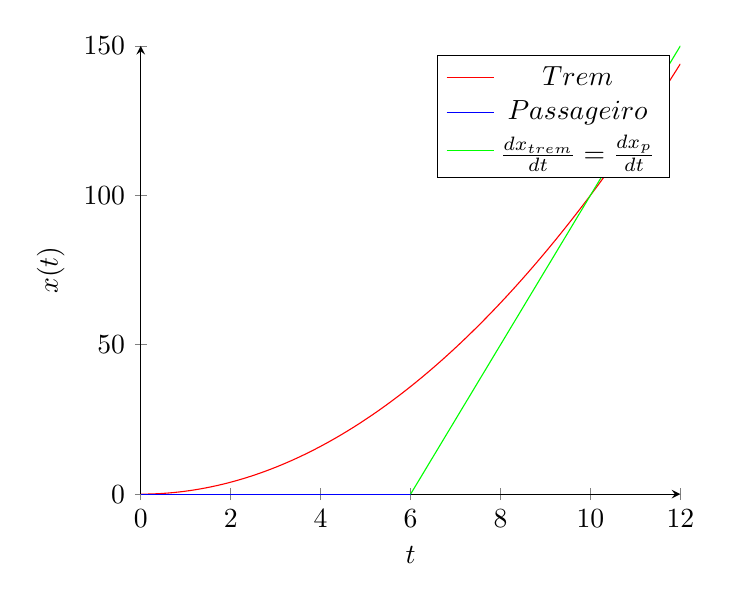
\begin{tikzpicture}
		\begin{axis}[
				axis lines = left,
				xlabel = \(t\),
				ylabel = {\(x(t)\)},
			]
			\addplot [
				domain=0:12,
				samples=100,
				color=red,
			]
			{x^2};
			\addlegendentry{\(\text{Trem}\)}
			\addplot[
				domain=0:6,
				samples=100,
				color=blue,
			]
			{0};
			\addlegendentry{\(\text{Passageiro}\)}
			\addplot[
				domain=6:12,
				samples=100,
				color=green,
			]
			{25*x-150};
			\addlegendentry{\(\frac{dx_{trem}}{dt} = \frac{dx_{p}}{dt}\)}
		\end{axis}
	\end{tikzpicture}
\end{center}
Ou seja, buscamos $t^{*}$ tal que $x_{p}(t^{*}) = x_{trem}(t^{*}), v_{p}(t^{*}) = v_{trem}(t^{*})$. Com efeito,
\begin{align*}
	v_{0}(t^{*} - 6) & = \frac{at^{*^{2}}}{2} \Rightarrow v_{0} = at^{*} \Rightarrow t^{*} = \frac{v_{0}}{a}                                                 \\
	                 & v_{0} = \frac{a}{2}\frac{(\frac{v_{0}}{a})^{2}}{\frac{v_{0}}{a}-6} \Rightarrow \frac{v_{0}^{2}}{2a} = 6v_{0} \Rightarrow v_{0} = 12a.
\end{align*}
Outra forma de resolver é utilizando o fato de que quando $\frac{dv}{dt} = 0$, a função está num mínimo. Ou seja, basta encontrar
o valor mínimo de $v_{0}$ que satisfaça o que buscamos. Temos
$$
	v_{0}(t-6) = \frac{at^{2}}{2} \Rightarrow v_{0}(t) = \frac{at^{2}}{2}\frac{1}{(t-6)}.
$$
Agora, derivando essa equação para $v_{0},$
$$
	\frac{dv_{0}}{dt} = \frac{d}{dt}\biggl(\frac{at^{2}}{2}\frac{1}{t-6}\biggr) = \frac{d}{dt}(f(t)g(t)),
$$
em que $f(t) = \frac{at^{2}}{2}, g(t) = (t-6)^{-1}$. Fazemos isso porque há uma regra para derivar o produto de funções,
a Regra do Produto
$$
	\boxed{\frac{df(t)g(t)}{dt}= g(t)\frac{df(t)}{dt} + f(t)\frac{dg(t)}{dt}}
$$
Derivando individualmente f e g,
$$
	\frac{df(t)}{dt} = at, \quad \frac{dg(t)}{dt} = -(t-6)^{-2} = -\frac{1}{(t-6)^{2}}.
$$
Agora, vamos juntar tudo para obter a derivada de $v_{0}$:
\begin{align*}
	\frac{dv_{0}}{dt} & = \frac{df(t)}{dt}g(t) + \frac{dg(t)}{dt}f(t) = \frac{at}{t-6} - \frac{1}{2(t-6)^{2}}at^{2} \\
	                  & = at\biggl(\frac{1}{t-6} - \frac{t}{2(t-6)^{2}}\biggr) = 0                                  \\
	                  & \Rightarrow \frac{1}{t-6} = \frac{t}{2(t-6)} \Rightarrow 1 = \frac{t}{2(t-6)}               \\
	                  & \Rightarrow 2(t-6) = t \Rightarrow 2t - t = 12 \Rightarrow t = 12s.
\end{align*}
\end{document}
